\documentclass[12pt]{scrartcl}
\usepackage{setspace}
\onehalfspacing
\usepackage{amsmath,amssymb,amsfonts,amsthm,mathtools}
\usepackage[english]{babel}
\usepackage[T1]{fontenc}
\usepackage[utf8x]{inputenc}
\usepackage{lmodern}
\usepackage{dsfont}
\usepackage{bbm}
\usepackage[round]{natbib}
\usepackage{color} 
\usepackage[defaultlines=2,all]{nowidow}
\usepackage{caption}
\usepackage[labelformat=simple]{subcaption}
\usepackage{hyperref} % Added for clickable links
\usepackage{placeins} % For FloatBarrier to prevent figures from floating past section boundaries
\usepackage{float} % For [H] placement specifier to force exact table/figure placement
\renewcommand\thesubfigure{(\alph{subfigure})}

% Set margin if needed, otherwise scrartcl default is used. 
% Standard academic reports often use geometry, but kept minimal here to match your original style.

\setlength\parindent{0pt}
\setlength{\parskip}{6pt plus 1pt minus 1pt}

\newcommand{\red}{\textcolor{red}}

\begin{document}

\begin{titlepage}
	\centering
	{\scshape\LARGE TU Dortmund \par}
	\vspace{1cm}
	{\scshape\Large On the Theory and Practice of Monte Carlo Simulations \par}
	\vspace{0.5cm}
	{\large Winter Semester 2025/26 \par}
	\vspace{2cm}
	{\huge\bfseries Final Project: Monte Carlo methods in reinforcement learning\par}
	\vspace{3cm}
	{\Large Author: Rohith B Chowdappa \par}
	\vspace{0.5 cm}
	{\large Student ID: 269962 \par}
	\vfill
	{\large Instructors: \par}
	{\large Prof. Dr. Katja Ickstadt \par}
	{\large Zeyu Ding \par}
	\vspace{1cm}
	{\large \today\par}
\end{titlepage}

\tableofcontents
\thispagestyle{empty}

\cleardoublepage

\setcounter{page}{1}

% Include all sections
% --- SECTION 1: INTRODUCTION ---
\section{Introduction}

Financial markets are complex, random, and highly volatile systems in which decision-making under uncertainty plays a central role. Designing trading strategies that can adapt to evolving market conditions remains a challenging problem due to noise, non-stationarity, and the absence of a known model governing price movement. Reinforcement learning (RL) offers a framework in which an agent learns directly from interaction with the environment and the data as opposed to traditional rule-based strategies \citep{hsinhungw2024}.

In this project, I investigate the use of Monte Carlo policy gradient methods for algorithmic trading within the gym-trading-env framework. The trading problem is formulated as a Markov Decision Process (MDP), where the agent observes market features derived from real historical data and decides between discrete actions (e.g., long, short, hold). The environment provides rewards based on portfolio performance, allowing the agent to iteratively improve its policy through experience.

The primary research question of this study is: \emph{Can a Monte Carlo policy gradient method (REINFORCE) learn a profitable and stable trading policy from historical market data, and how does its performance compare to baseline strategies such as random trading?}

Monte Carlo (MC) methods are particularly appropriate for this problem for several reasons. First, financial returns are inherently noisy and difficult to model analytically. MC RL does not require an explicit transition model of the market; instead, it estimates expected returns directly from sampled trajectories. Second, policy gradient methods optimize the policy parameters directly, making them well-suited for high-dimensional continuous state spaces typical of financial time series. Third, Monte Carlo estimation produces unbiased return estimates, enabling a theoretically grounded analysis of convergence behavior, albeit with potentially high variance.

In this project, I implement the REINFORCE algorithm \citep{williams1992simple} using a neural network policy (multi-layer perceptron with softmax output) to model a stochastic trading strategy. The agent is trained on historical market data, and policy updates are performed at the end of each episode using the discounted return. To reduce variance in gradient estimates, a variant of the same alogorithm was introduced, these two main methods was then compared to a random trading strategy which acts as a benchmark.
% --- SECTION 2: THEORETICAL BACKGROUND ---
\section{Theoretical Background}

\subsection{Reinforcement Learning Framework}

The trading problem is formulated as a Markov Decision Process (MDP), defined by the tuple 
$(\mathcal{S}, \mathcal{A}, P, R, \gamma)$, where $\mathcal{S}$ denotes the state space, 
$\mathcal{A}$ the action space, $P$ the transition dynamics, $R$ the reward function, and 
$\gamma \in (0,1)$ the discount factor.

At each time step $t$, the agent observes a state $s_t$ (constructed from market features), 
selects an action $a_t$ according to a parameterized stochastic policy $\pi_\theta(a|s)$, 
receives reward $r_{t+1}$, and transitions to the next state $s_{t+1}$.

The reward function is defined as the logarithmic return of the portfolio valuation:
\[
r_t = \ln\left(\frac{p_t}{p_{t-1}}\right),
\]
where $p_t$ denotes the portfolio valuation at time step $t$.

The objective is to maximize the expected discounted return:

\[
J(\theta) = \mathbb{E}_{\pi_\theta} 
\left[ 
\sum_{t=0}^{T} \gamma^t r_{t+1} 
\right].
\]

In contrast to value-based methods, policy gradient approaches directly optimize 
the policy parameters $\theta$ to increase expected return \citep{wikipediapolicysradient}.

\subsection{Monte Carlo Policy Gradient (REINFORCE)}

Monte Carlo methods estimate returns using complete sampled episodes. 
For a trajectory of length $T$, the return from time step $t$ is defined as:

\[
G_t = \sum_{k=0}^{T-t} \gamma^k r_{t+k+1}.
\]

Unlike temporal-difference methods, Monte Carlo approaches do not use bootstrapping; 
they rely solely on actual observed rewards. This leads to unbiased return estimates, 
but potentially high variance.

Using the log-derivative trick, the gradient of the objective function can be written as:

\[
\nabla_\theta J(\theta) =
\mathbb{E}_{\pi_\theta}
\left[
G_t \nabla_\theta \log \pi_\theta(a_t|s_t)
\right].
\]

This result leads to the REINFORCE update rule \citep{williams1992simple}:

\[
\theta \leftarrow \theta 
+ \alpha \, G_t \nabla_\theta \log \pi_\theta(a_t|s_t),
\]

where $\alpha$ is the learning rate.

In practice, the expectation is approximated using sampled trajectories. 
Updates are performed after each episode, making the algorithm fully Monte Carlo.

\subsection{Variance and Baseline Reduction}

A key limitation of REINFORCE is the high variance of its gradient estimator. 
In financial environments, rewards are noisy and highly volatile, which can 
lead to unstable learning and slow convergence.

To reduce variance without introducing bias, a baseline function $b(s_t)$ 
can be subtracted from the return:

\[
\nabla_\theta J(\theta)
=
\mathbb{E}
\left[
(G_t - b(s_t)) \nabla_\theta \log \pi_\theta(a_t|s_t)
\right].
\]

If the baseline depends only on the state and not on the action, 
the estimator remains unbiased. A common choice is the state-value function 
$V(s_t)$, which estimates the expected return from state $s_t$.

Defining the advantage as

\[
A_t = G_t - V(s_t),
\]

the update becomes:

\[
\theta \leftarrow \theta 
+ \alpha \, A_t \nabla_\theta \log \pi_\theta(a_t|s_t).
\]

The subtraction centers the gradient signal around zero, 
reducing variance and improving stability. 

In this project, the performance of standard REINFORCE 
is compared to REINFORCE with a learned value-function baseline. 
The comparison focuses on convergence behavior and training stability 
in a noisy financial environment.


\subsection{Practical Stabilization Techniques}
\label{sec:stabilization}

To address instability and high variance in neural network-based reinforcement learning \citep{wikipediapolicysradient}, these techniques were implemented:

\begin{enumerate}
    \item \textbf{Return Normalization:}
    \[
    \hat{G}_t = \frac{G_t - \mu_G}{\sigma_G + \epsilon}
    \]
    Normalizing returns reduces fluctuations in gradient scale, which helps stabilize neural network training, especially when episodic returns can be highly volatile.

    \item \textbf{Gradient Clipping:} \\
    To prevent exploding gradients during backpropagation, the norm of the gradient $g$ is clipped to a maximum value $c$:
    \[
    \|g\| \leq c
    \]
    This ensures stable policy updates.

    \item \textbf{Softmax Policy Parameterization:} \\
    The policy is typically parameterized using a softmax over action preferences to guarantee a valid probability distribution:
    \[
    \sum_a \pi_\theta(a|s) = 1
    \]
    This preserves sufficient exploration and prevents the policy from collapsing to deterministic actions too early.
\end{enumerate}

These stabilization techniques are essential for robust RL training in noisy financial domains.

% --- SECTION 3: DATA DESCRIPTION ---
\section{Data Description}

The dataset used in this study was obtained from Kaggle \citep{kaggle2024} and contains daily historical price data at a one-day interval for all working days for major stock market indices worldwide. The data were originally collected from Yahoo Finance and span several decades (1965–2021). For this project, we selected the German stock market index \textbf{GDAXI (DAX)}, which represents the 40 largest blue-chip companies traded on the Frankfurt Stock Exchange. The DAX serves as a benchmark index for the German equity market and is widely used in financial research due to its liquidity and economic significance.

Although the dataset provides a long historical record, computational constraints required restricting the analysis to a more recent subset. Therefore, we selected the period from January 2016 to December 2021. After filtering and removing missing values introduced during preprocessing, the final dataset consists of 1,369 daily observations. This time window includes multiple market conditions, such as bullish trends, market corrections, and the COVID-19 crisis, thereby providing sufficient variability for RL experiments.

To ensure compatibility with the trading environment, the dataset was structured by sorting observations in ascending chronological order and converting the date column into a \texttt{DatetimeIndex}. The dataset contains standard OHLCV columns including \texttt{open}, \texttt{high}, \texttt{low}, \texttt{close}, \texttt{adj close}, and \texttt{volume}.

To enhance the state representation provided to the reinforcement learning agent, a small number of additional features were engineered. These include:

\begin{itemize}
    \item Daily log returns (momentum information)
    \item Rolling volatility (short-term risk estimate)
    \item Moving average ratio (trend indicator)
    \item Normalized trading volume (activity indicator)
\end{itemize}

All engineered features were normalized to stabilize neural network training.
% --- SECTION 4: EMPIRICAL RESULTS ---
\section{Empirical Results}

\subsection{Implementation Details}

The Monte Carlo reinforcement learning agent was implemented in \textbf{Python 3.10} using the following key libraries:

\begin{itemize}
    \item \texttt{PyTorch} for neural network policy and value function implementation
    \item \texttt{NumPy} and \texttt{Pandas} for data manipulation and feature engineering
    \item \texttt{gym-trading-env} as the trading environment
    \item \texttt{Matplotlib} and \texttt{Seaborn} for visualization of learning curves and results
\end{itemize}

\subsubsection{Environment Setup}
Gym Trading Env \citep{gymtradingenv} is a Gymnasium environment for simulating stocks and training Reinforcement Learning (RL) trading agents. It was designed to be fast and customizable for easy RL trading algorithms implementation. The trading environment was configured to simulate daily trading on the DAX index using the preprocessed dataset described in Section 3.

To ensure robustness, the agents were trained using \textbf{10 different random seeds}. This allows for an assessment of variability in learning outcomes and provides reliable statistical estimates of agent performance. 

\subsubsection{Neural Network Architecture and Hyperparameters}
The policy network consists of two fully connected hidden layers with 128 units each, using ReLU activation functions. The network outputs action probabilities via a softmax layer. For the baseline variant, a separate value network with identical architecture (except for a single output unit) estimates state values. Both networks are optimized using the \textbf{Adam} optimizer with a learning rate of \textbf{1e-3} and a discount factor $\gamma = 0.99$. Gradient clipping with a maximum norm of 1.0 is applied to stabilize training, and returns are normalized before computing policy gradients to reduce variance.

\begin{figure}[htbp]
    \centering
    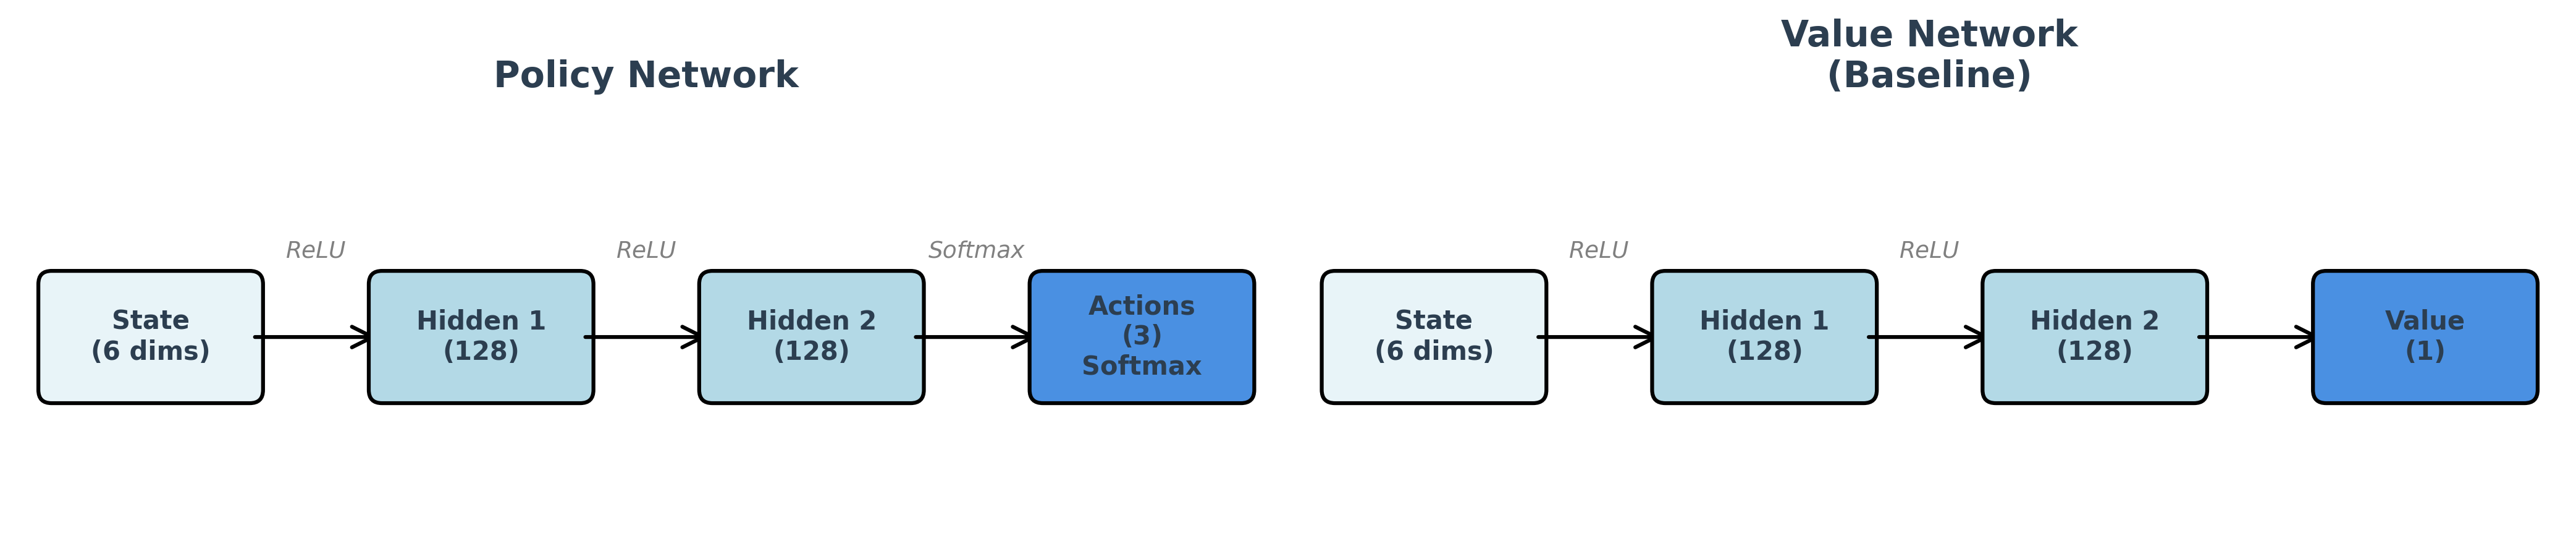
\includegraphics[width=0.8\textwidth]{../report/figures/model_architecture.png}
    \caption{Overview of the neural network architecture for the REINFORCE agent. The policy network (left) maps states to action probabilities, while the value network (right, used in the baseline variant) estimates state values.}
    \label{fig:model_architecture}
\end{figure}


\subsection{Empirical Results}

This section presents the empirical findings of the Monte Carlo policy gradient agents trained on historical DAX data. 
The methods compared are REINFORCE without baseline, REINFORCE with a learned value-function baseline, 
and a random trading strategy serving as a lower-bound benchmark.

\subsubsection{Learning Dynamics and Convergence}

\begin{figure}[htbp]
    \centering
    \begin{subfigure}[t]{0.48\textwidth}
        \centering
        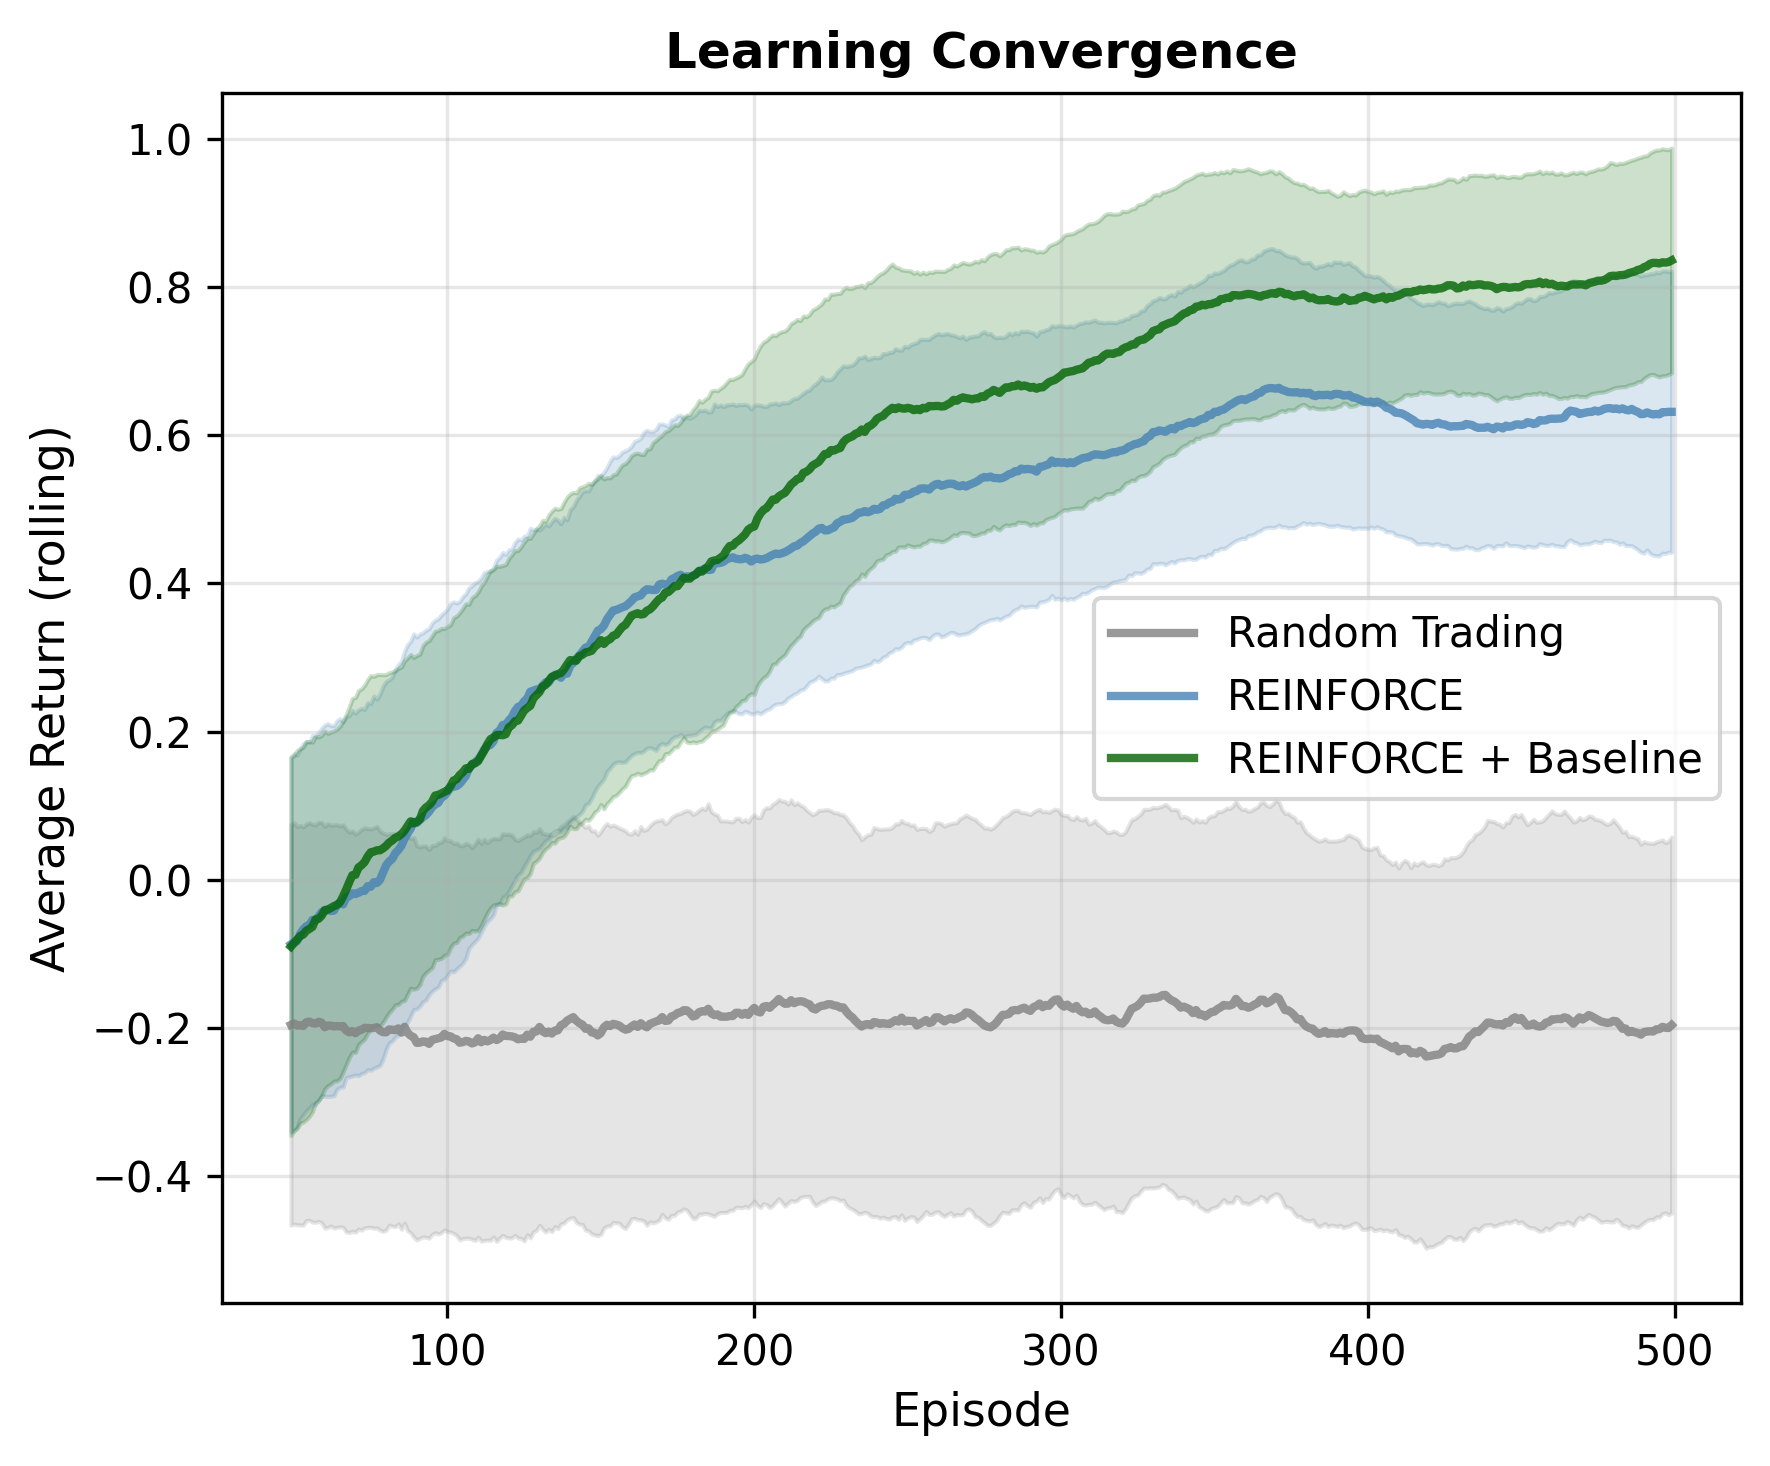
\includegraphics[width=\textwidth]{../report/figures/convergence_convergence.png}
        \caption{Learning convergence: Rolling average episode return across 10 random seeds.}
        \label{fig:learning_convergence}
    \end{subfigure}
    \hfill
    \begin{subfigure}[t]{0.48\textwidth}
        \centering
        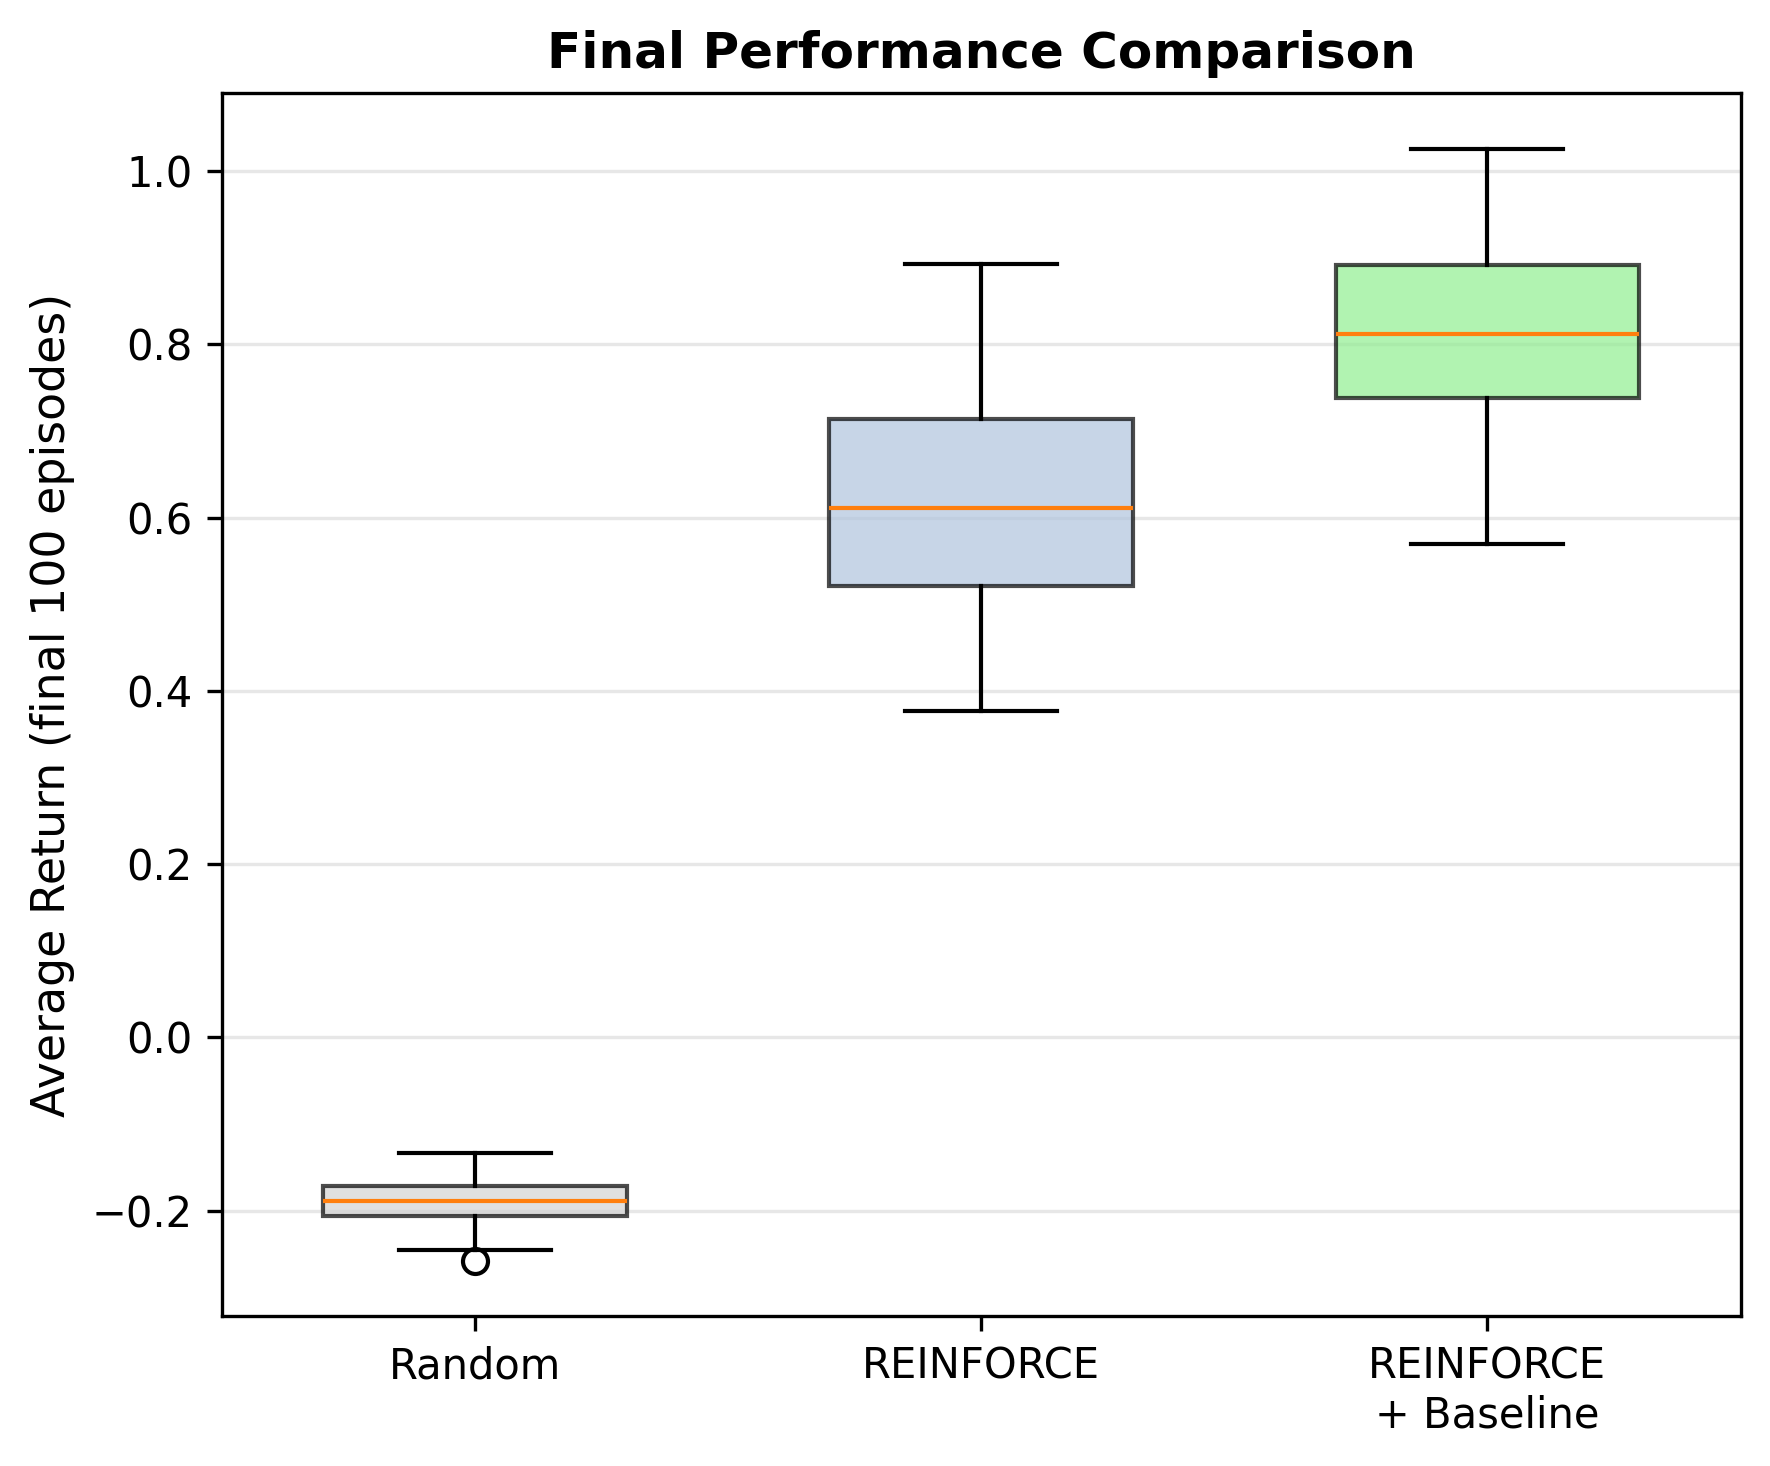
\includegraphics[width=\textwidth]{../report/figures/convergence_final_performance.png}
        \caption{Boxplot comparing average returns in the final 100 episodes.}
        \label{fig:performance_comparison}
    \end{subfigure}
\end{figure}


Figure~\ref{fig:learning_convergence} shows the rolling average return per episode. 
The REINFORCE agent with baseline converges faster and exhibits smoother learning curves compared to 
the standard REINFORCE agent. This supports the theoretical expectation that incorporating a value-function baseline 
reduces gradient variance and stabilizes learning.

Figure~\ref{fig:performance_comparison} presents a boxplot of the average return over the final 100 episodes. 
The baseline variant achieves higher median returns and a narrower interquartile range, 
indicating improved performance and reduced variability across seeds. 
The random policy displays the dispersion centered around -0.2, confirming its role as a benchmark 
without learning capability.

\subsubsection{Return Distribution and Risk Analysis}

\begin{figure}[htbp]
    \centering
    \begin{subfigure}[t]{0.48\textwidth}
        \centering
        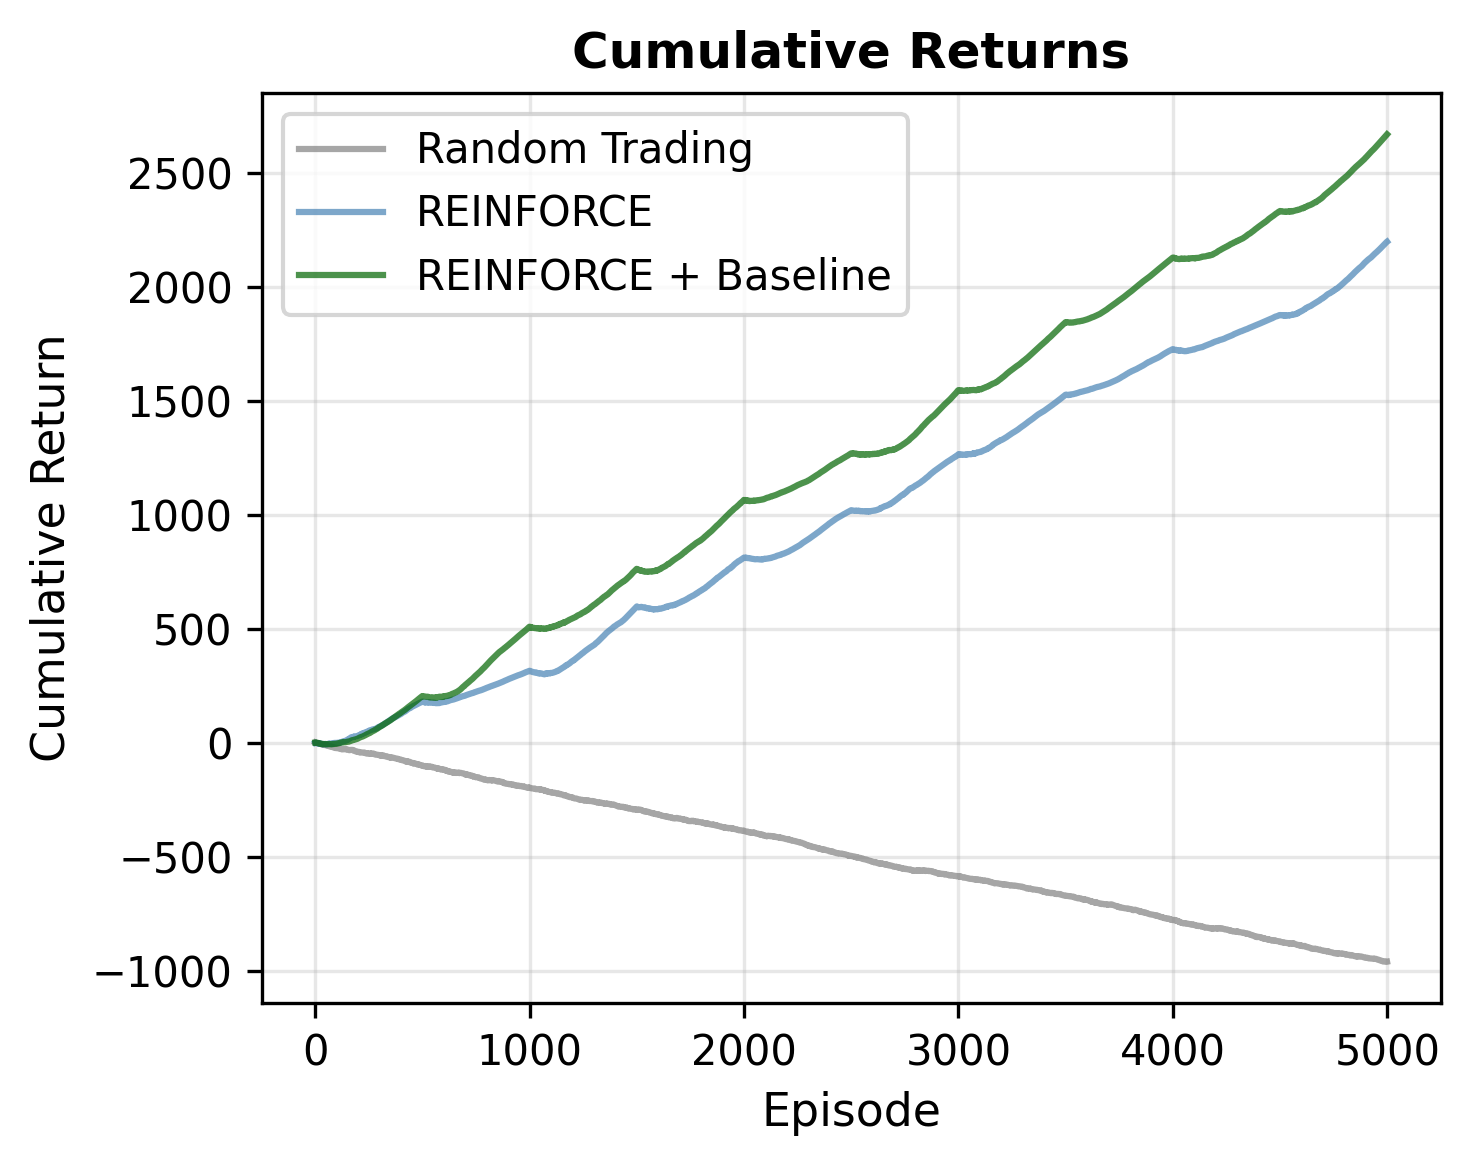
\includegraphics[width=\textwidth]{../report/figures/return_cumulative.png}
        \caption{Distribution of episode returns across 10 random seeds.}
        \label{fig:cumulative_return}
    \end{subfigure}
    \hfill
    \begin{subfigure}[t]{0.48\textwidth}
        \centering
        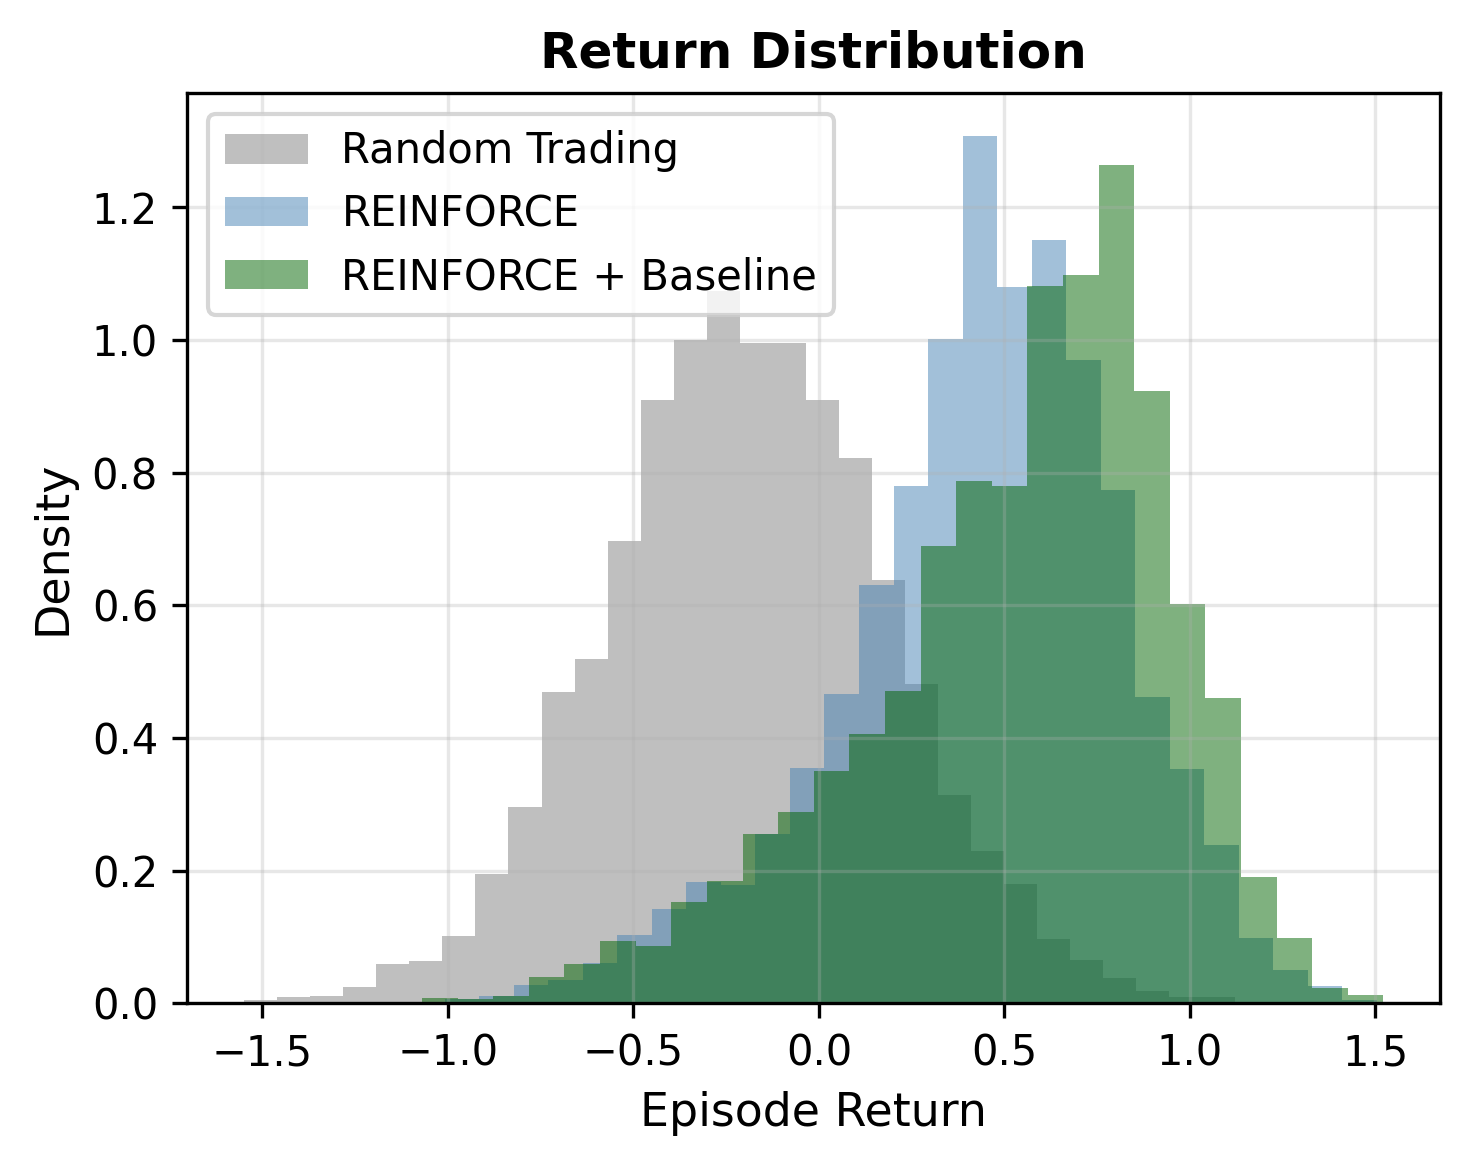
\includegraphics[width=\textwidth]{../report/figures/return_distribution.png}
        \caption{Cumulative portfolio return over the evaluation period.}
        \label{fig:return_distribution}
    \end{subfigure}
\end{figure}


Figure~\ref{fig:cumulative_return} presents cumulative portfolio performance. 
Both Monte Carlo agents achieve sustained positive growth, with the baseline variant showing 
a smoother trajectory and higher overall gains. In contrast, the random strategy demonstrates 
a steady downward trend, indicating no systematic profitability.

Figure~\ref{fig:return_distribution} shows the distribution of episode returns. 
REINFORCE with a baseline yields a tighter distribution concentrated around positive returns, 
indicating lower variance. The standard REINFORCE agent exhibits greater dispersion with occasional 
negative outcomes. The random policy is centered slightly below zero, reflecting the 
absence of learning and a tendency toward marginal losses.

\subsubsection{Summary of Quantitative Metrics}

\FloatBarrier % Prevent previous floats from interfering with table placement
\begin{table}[H]
\centering
\caption{Performance comparison across methods (averaged over 10 seeds).}
\label{tab:performance}
\resizebox{0.95\textwidth}{!}{%
\begin{tabular}{lcccccc}
\hline
Method & Mean Return & Std Dev & 95\% CI & SharpeRatio & Win Rate \\
\hline
REINFORCE+Baseline &  0.8177  &  0.1360 & [0.7204, 0.9149] & 20.5163 &  88.06  \\
REINFORCE & 0.6231 & 0.1745 & [0.4983, 0.7480] & 18.6067 & 87.94 \\
Random Policy &  -0.1925 & 0.0379 & [-0.2197, -0.1654] & -8.0677 & 30.48  \\

\hline
\end{tabular}%
}
\end{table}

Table~\ref{tab:performance} summarizes the key evaluation metrics, including mean final return, 
standard deviation, 95\% confidence interval, Sharpe ratio, and win rate (in percentage). 
The quantitative results confirm the visual evidence from the figures: 
REINFORCE with baseline consistently achieves higher returns, improved risk-adjusted performance, 
and reduced variability relative to standard REINFORCE. 
Both learning-based approaches substantially outperform the random trading strategy.

The confidence intervals show that both REINFORCE methods achieve positive returns, while the random policy does not. REINFORCE with a baseline has higher and more consistent returns, showing it learns a profitable and stable trading policy from historical data.

\FloatBarrier % Prevent figures from floating into the next section

\FloatBarrier % Ensure all figures from empirical results are placed before conclusion
% --- SECTION 5: CONCLUSION ---
\section{Conclusion and Discussion}

This study found that Monte Carlo policy gradient methods, specifically the REINFORCE algorithm, can learn profitable and systematic trading strategies from historical DAX index data and consistently outperform random trading. Empirical results showed that the use of a value-function baseline further improved performance by reducing variance and enhancing risk-adjusted returns, demonstrating the robustness and effectiveness of these methods for financial trading tasks.

\subsection*{Limitations}

Despite promising results, several limitations remain. The analysis focused solely on the DAX index, limiting generalizability to other assets or markets. The approach was also computationally expensive, and the state representation relied on simple engineered features. Furthermore, reinforcement learning in finance is inherently difficult due to non-stationarity, structural breaks, and noisy reward signals.

\subsection*{Future Work}

Future work could take several directions. For example, it would be useful to test these methods on multiple assets at once and let the agent choose how to split money across them, not just trade one index. It would also make the experiments more realistic to include trading costs and add more rules to limit risk.

Another possible step is to integrate large language models with these trading methods. For example, recent work has explored using language models to assist in live trading with real money while adhering to strict risk protocols \citep{llmtradinglab2024}. Combining language models with simple trading rules could make automated trading systems both smarter and safer.

In conclusion, this study demonstrates the viability of Monte Carlo policy gradient methods \citep{williams1992simple} for financial trading tasks. 
While further work is required to ensure robustness, 
the integration of reinforcement learning \citep{hsinhungw2024} with emerging large language model frameworks 
represents a promising direction for future research.




% --- BIBLIOGRAPHY ---
\newpage
\addcontentsline{toc}{section}{Bibliography}
\renewcommand\refname{Bibliography} 
\bibliographystyle{plainnat}
\bibliography{sections/references} % Make sure you have a references.bib file


% --- APPENDICES ---
\newpage
\appendix 
\addsec{Appendix}

\section*{A \ AI Usage Declaration}

\emph{I declare that I used ChatGPT (OpenAI GPT-4) to assist with structuring the report, 
improving clarity of explanations, and polishing the 
academic writing of several sections. In addition it was used to refactor, add inline documentation and to improve the readability of the code.}

\emph{In addition cursor agents were used to suggest improvements in section organization, 
to help draft interpretations of figures and tables based on results I had already generated, 
refining LaTeX formatting, and to assist in wording the discussion and future work sections.}

\emph{The design of the research question, data preprocessing, feature engineering, 
implementation of the reinforcement learning algorithms, experimental setup, 
statistical evaluation are entirely my own work. All final decisions regarding methodology, analysis, and conclusions were made independently by me.}



\end{document}

